\chapter{الجزيئات الحيوية: الأحماض الأمينية والسكريات والليبيدات والنوكليوتيدات}\label{ch:b2:biomolecules}

مُحلٍّ شائع، أحلى بكثير من السكر، هو حمضان أمينيان تصل بينهما رابطة أميد واحدة، وأحدهما
على هيئة إستره الميثيلي: حمض الأسبارتيك والفينيل ألانين، وكلاهما بالترتيب الفراغي الذي تستعمله
الخلايا الحية. وجزيئات الحياة مبنية من عائلات قليلة من الوحدات الصغيرة، الأحماض الأمينية والسكريات \omterm{def:b2:biomolecules:lipid}{والأحماض
الدهنية} \omterm{def:b2:biomolecules:nucleotide}{والنوكليوتيدات}، موصولة بتفاعلات الفصول السابقة: الأميدات، والأسيتالات، والإسترات. ويقرؤها
هذا الفصل كما يقرؤها الكيميائي العضوي: المجموعات الوظيفية، والكيمياء الفراغية، والسلوك
الحمضي--القاعدي، والتفاعلات التي تصلها وتقطعها.
% ledger: use:aspartame

\begin{recall}
مجلد السنة الأولى: قواعد CIP، وإسقاطات فيشر، والكيرالية، ونصف الأسيتالات والأسيتالات، و$\mathrm pK_a$
ومخططات التوزيع، والجزيئات الأمفيفيلية، وقانون بيو. و\cref{ch:b2:acyl-substitution}: الأميدات،
والإسترات، \omterm{def:b2:acyl-substitution:saponification}{والتصبّن}، والأحماض المنشطة. و\cref{ch:b2:amines}: الأمينات بوصفها قواعد.
و\cref{ch:b2:retrosynthesis}: المجموعات الحامية في طريق تخليقي.
\end{recall}

\section{الأحماض الأمينية}

\begin{definition}[الأحماض الأمينية]\label{def:b2:biomolecules:amino-acid}
\emph{الحمض الأميني $\alpha$}\index{حمض أميني ألفا@حمض أميني $\alpha$} \ce{H2N-CHR-COOH} يحمل
مجموعة أمينية ومجموعة حمض كربوكسيلي على الكربون نفسه؛ و\ce{R} هي \emph{سلسلته
الجانبية}\index{سلسلة جانبية}. وفي الماء قرب الأس الهيدروجيني المتعادل يوجد على هيئة \emph{أيون مزدوج الشحنة}\index{أيون مزدوج الشحنة}،
\ce{H3N+-CHR-COO-}، يحمل شحنة موجبة وأخرى سالبة. و\emph{نقطة التعادل
الكهربائي}\index{نقطة التعادل الكهربائي} pI هي قيمة pH التي تنعدم عندها شحنته الصافية المتوسطة.
\end{definition}

عشرون حمضًا أمينيًا تبني بروتينات الكائنات الحية. وكلها كيرالية ما عدا الغليسين (\ce{R = H})، 
وللطبيعية منها الترتيب L (\cref{def:b2:biomolecules:d-l}). وتصنّفها سلاسلها الجانبية
عائلات: غير قطبية (الألانين، \ce{R = CH3}؛ والفينيل ألانين، \ce{R = CH2C6H5})، وقطبية، وحمضية
(حمضا الأسبارتيك والغلوتاميك، بمجموعة كربوكسيلية ثانية) وقاعدية (الليسين، بمجموعة أمينية
ثانية؛ والهستيدين، بحلقة إيميدازول).

\begin{proposition}[نقطة التعادل الكهربائي]\label{prop:b2:biomolecules:pi}
من أجل حمض أميني \omterm{def:b2:biomolecules:amino-acid}{سلسلته الجانبية} ليست حمضية ولا قاعدية، $\mathrm{pI} = (\mathrm pK_{a1} +
\mathrm pK_{a2})/2$، حيث $\mathrm pK_{a1}$ للمجموعة الكربوكسيلية و$\mathrm pK_{a2}$ لمجموعة
الأمونيوم. ومن أجل \omterm{def:b2:biomolecules:amino-acid}{سلسلة جانبية} حمضية أو قاعدية، تكون pI متوسط قيمتي $\mathrm pK_a$ اللتين تحيطان
بالصورة المتعادلة.
\end{proposition}

\begin{proof}
لنكتب \ce{H2A+} للكاتيون، و\ce{HA} \omterm{def:b2:biomolecules:amino-acid}{للأيون المزدوج الشحنة} و\ce{A-} للأنيون. تنعدم الشحنة الصافية
حين $[\ce{H2A+}] = [\ce{A-}]$. ومن $K_{a1} = [\ce{HA}]h/[\ce{H2A+}]$ و$K_{a2} =
[\ce{A-}]h/[\ce{HA}]$، مع $h = [\ce{H3O+}]$، تكون النسبة $[\ce{H2A+}]/[\ce{A-}] = h^2/(K_{a1}K_{a2})$
مساوية 1 من أجل $h^2 = K_{a1}K_{a2}$، أي $\mathrm{pH} = (\mathrm pK_{a1} + \mathrm pK_{a2})/2$. ومع
مجموعة ثالثة قابلة للتأين ينطبق التعليل نفسه على التوازنين الواقعين على جانبي الصورة
المتعادلة، إذ تكون المجموعة الثالثة حينئذ كليًا في حالة واحدة.
\end{proof}

من أجل الغليسين، $\mathrm pK_{a1} = 2.35$ و$\mathrm pK_{a2} = 9.78$: pI $\approx 6.1$. ولحمض الأسبارتيك
(2.0، 3.9، 9.9) pI $\approx 3.0$؛ ولليسين (2.2، 9.1، 10.7) pI $\approx 9.9$.
% ledger: pka:glycine1, pka:glycine2, pka:asp1, pka:asp2, pka:asp3, pka:lys1, pka:lys2, pka:lys3

\begin{omfigure}
\begin{tikzpicture}
\begin{axis}[width=0.47\linewidth, height=5cm, xmin=0, xmax=14, ymin=-2.2, ymax=2.2,
  xlabel={\babelsublr{pH}}, ylabel={\foreignlanguage{arabic}{الشحنة الصافية}}, label style={font=\small}, tick label style={font=\scriptsize},
  xtick={0,2,4,6,8,10,12,14}, ytick={-2,-1,0,1,2}, grid=major, grid style={black!12},
  legend style={font=\scriptsize, at={(0.5,1.03)}, anchor=south}, legend columns=3]
\addplot[omDef, thick] table[x=pH, y=gly] {figdata/out/bachelor-2-amino-acid-charge-a.dat};
\addplot[omThm, thick] table[x=pH, y=asp] {figdata/out/bachelor-2-amino-acid-charge-a.dat};
\addplot[omMeth, thick] table[x=pH, y=lys] {figdata/out/bachelor-2-amino-acid-charge-a.dat};
\legend{غليسين, حمض الأسبارتيك, ليسين}
\end{axis}
\end{tikzpicture}\hfill
\begin{tikzpicture}
\begin{axis}[width=0.47\linewidth, height=5cm, xmin=0, xmax=14, ymin=0, ymax=1.05,
  xlabel={\babelsublr{pH}}, ylabel={الكسر}, label style={font=\small}, tick label style={font=\scriptsize},
  xtick={0,2,4,6,8,10,12,14},
  legend style={font=\scriptsize, at={(0.5,1.03)}, anchor=south}, legend columns=3]
\addplot[omThm, thick] table[x=pH, y=cation] {figdata/out/bachelor-2-amino-acid-charge-b.dat};
\addplot[omDef, thick] table[x=pH, y=zwitterion] {figdata/out/bachelor-2-amino-acid-charge-b.dat};
\addplot[omMeth, thick] table[x=pH, y=anion] {figdata/out/bachelor-2-amino-acid-charge-b.dat};
\legend{كاتيون, أيون مزدوج الشحنة, أنيون}
\end{axis}
\end{tikzpicture}

{\small يمينًا: الشحنة الصافية لثلاثة أحماض أمينية بدلالة pH، انطلاقًا من قيم $\mathrm pK_a$ لها عند
\qty{25}{\degreeCelsius}؛ وكل منحنى يقطع الصفر عند pI. يسارًا: صور الغليسين الثلاث،
\ce{H3N+CH2COOH} و\ce{H3N+CH2COO-} و\ce{H2NCH2COO-}؛ ويسود \omterm{def:b2:biomolecules:amino-acid}{الأيون المزدوج الشحنة} من نحو pH 3 إلى
pH 9.}
% figdata: bachelor-2/amino-acid-charge.py parts a, b
\end{omfigure}

\begin{method}[الشحنة الصافية عند pH معلوم]\label{met:b2:biomolecules:charge}
\begin{enumerate}
  \item عدّد كل مجموعة قابلة للتأين مع $\mathrm pK_a$ لها: \ce{NH3+} و\ce{COOH} الطرفيتين، 
        والسلاسل الجانبية القابلة للتأين.
  \item لكل مجموعة، قارن pH و$\mathrm pK_a$: تكون المجموعة مبرتنة في الغالب تحت
        $\mathrm pK_a$ لها، ومنزوعة البروتون في الغالب فوقها (وبأكثر من وحدة واحدة: فوق 90~\%).
  \item اجمع الشحنات: \ce{NH3+} $+1$، \ce{NH2} 0، \ce{COOH} 0، \ce{COO-} $-1$ (الإيميدازوليوم $+1$).
  \item قرب $\mathrm pK_a$ ما، احسب تلك المجموعة نصف مشحونة؛ وللحصول على قيمة مضبوطة، استعمل الكسور
        $1/(1 + 10^{\mathrm pK_a - \mathrm{pH}})$.
\end{enumerate}
\end{method}

\section{الببتيدات}

\begin{definition}[الببتيدات]\label{def:b2:biomolecules:peptide}
رابطة الأميد المتكوّنة بين المجموعة الكربوكسيلية لحمض أميني والمجموعة الأمينية لآخر هي
\emph{رابطة ببتيدية}\index{رابطة ببتيدية}؛ وسلسلة الأحماض الأمينية الموصولة بروابط ببتيدية هي
\emph{ببتيد}\index{ببتيد} (وبروتين حين تكون طويلة)، يُكتب من طرفه الأميني الحر (الطرف N)
إلى طرفه الكربوكسيلي الحر (الطرف C). و\emph{الاقتران الببتيدي}\index{اقتران ببتيدي} يكوّن
رابطة ببتيدية في المختبر بواسطة \emph{عامل اقتران}\index{عامل اقتران}، وهو كاشف
يحوّل المجموعة الكربوكسيلية إلى مشتق منشط في ظروف لطيفة (كربوديإيميد، مثلًا).
\end{definition}

\begin{omfigure}
\setchemfig{atom sep=1.9em}
\schemestart
\chemfig{R-C(=[2]O)-N(-[6]H)-R'}
\arrow{<->}
\chemfig{R-C(-[2]\chemabove{O}{\scriptstyle -})=\chemabove{N}{\scriptstyle +}(-[6]H)-R'}
\schemestop
\par\vspace{6pt}

{\small بنيتا الرنين \omterm{def:b2:biomolecules:peptide}{للرابطة الببتيدية}. يتقاسم الزوج الحر للنيتروجين مع
الكربونيل: فللرابطة \ce{C-N} طابع جزئي لرابطة مزدوجة، وتقع الذرات الست C وC وO وN وH وC
في مستوٍ واحد.}
\end{omfigure}

\begin{proposition}[رابطة مستوية]\label{prop:b2:biomolecules:planar}
\omterm{def:b2:biomolecules:peptide}{الرابطة الببتيدية} مستوية، والدوران حول الرابطة \ce{C-N} مقيد، ونيتروجين الأميد
ليس قاعديًا ولا محبًا للنواة.
\end{proposition}

\begin{proof}[تعليل]
بنية الرنين الثانية تعطي الرابطة \ce{C-N} نصيبًا من طابع الرابطة المزدوجة: فتدويرها
يقطع تداخل الزوج الحر للنيتروجين مع نظام $\pi$ في \ce{C=O}، وهو ما يكلف طاقة، فتبقى
الذرات المحيطة بها في مستوٍ واحد، والترتيب trans (كربونا السلسلة في جهتين متقابلتين من
الرابطة \ce{C-N}) هو المعتاد. والزوج الحر المنخرط في الرنين غير متاح لبروتون أو
لمحب للإلكترونات، كما في كل أميد (\cref{ch:b2:acyl-substitution}). وتنطوي البروتينات حول سلاسل من هذه
المستويات الصلبة.
\end{proof}

\begin{proposition}[لماذا الحماية والتنشيط]\label{prop:b2:biomolecules:coupling}
يتطلب صنع ثنائي \omterm{def:b2:biomolecules:peptide}{ببتيد} معيّن من حمضين أمينيين حماية المجموعات التي يجب ألا
تتفاعل وتنشيط المجموعة الكربوكسيلية التي يجب أن تتفاعل.
\end{proposition}

\begin{proof}[تعليل]
الحمض الكربوكسيلي والأمين المخلوطان في درجة حرارة الغرفة يعطيان ملحًا، لا أميدًا؛ والتسخين لطرد
الماء كان سيحوّل الأحماض الأمينية أيضًا إلى راسيمية. فيلزم التنشيط (\omterm{def:b2:acyl-substitution:derivative}{كلوريد أسيل}، أو أنهيدريد، أو \omterm{def:b2:biomolecules:peptide}{عامل
اقتران}). لكن لكل حمض أميني المجموعتين كلتيهما: فتنشيط خليط من الغليسين 
والألانين كان سيعطي Gly--Ala وAla--Gly وGly--Gly وAla--Ala وسلاسل أطول. وحجب أمين
الأول وحمض الثاني لا يترك إلا رابطة واحدة ممكنة.
\end{proof}

\begin{method}[تخليق ثنائي ببتيد]\label{met:b2:biomolecules:peptide}
\begin{enumerate}
  \item احمِ المجموعة الأمينية للحمض الأميني الطرفي N (على هيئة كربامات، مثلًا مجموعة
        \textit{tert}-بيوتوكسي كربونيل).
  \item احمِ المجموعة الكربوكسيلية للحمض الأميني الطرفي C (على هيئة إستر ميثيلي أو بنزيلي)، وكل
        \omterm{def:b2:biomolecules:amino-acid}{سلسلة جانبية} تفاعلية.
  \item نشّط المجموعة الكربوكسيلية الحرة \omterm{def:b2:biomolecules:peptide}{بعامل اقتران} وأضف الشريك المحمي: فتتكوّن \omterm{def:b2:biomolecules:peptide}{رابطة
        ببتيدية} واحدة.
  \item أزل المجموعات الحامية، ويُفضَّل أن تكون مجموعة متعامدة
        (\cref{def:b2:retrosynthesis:orthogonal})؛ وللاستمرار، أزل حماية الأمين وحدها وكرر.
\end{enumerate}
\end{method}

تكرار الدورة مرات كثيرة في المحلول كان سيتطلب تنقية عند كل خطوة. أما في التخليق
على الطور الصلب، فتُربط السلسلة النامية بطرفها C إلى حبيبة بوليمرية؛ وتُغسل الكواشف الزائدة 
والنواتج الثانوية بعد كل اقتران، ويُقطع \omterm{def:b2:biomolecules:peptide}{الببتيد} المكتمل عن الحامل في
النهاية.

\begin{omfigure}
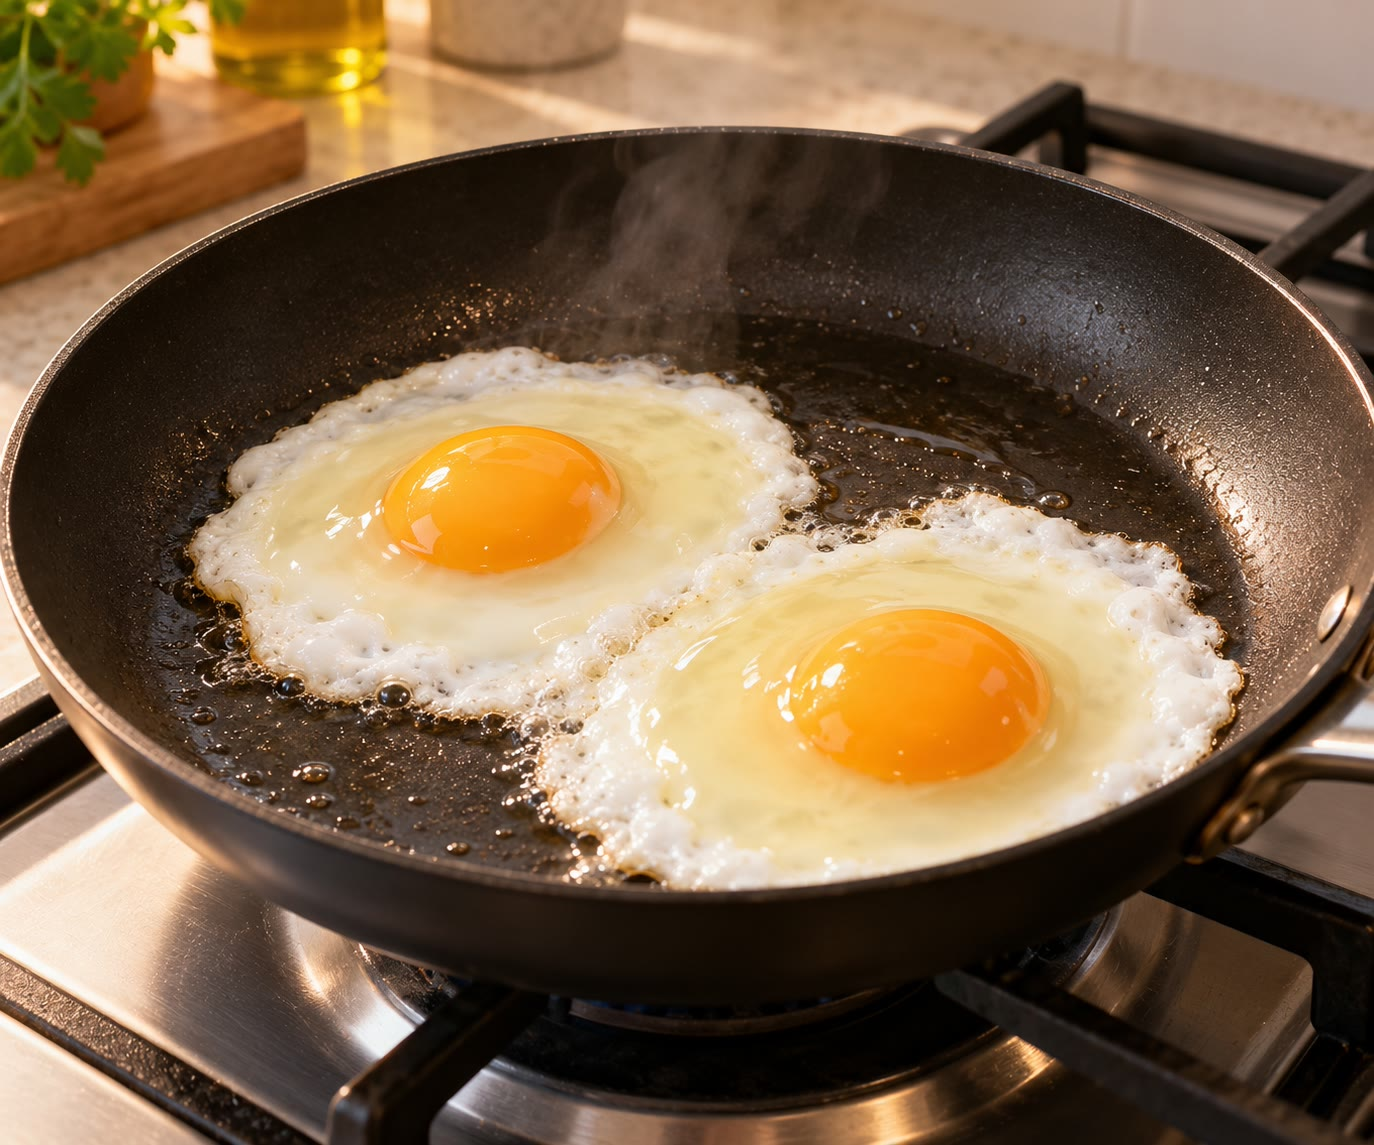
\includegraphics[width=0.5\linewidth]{images/book3/ai/b2-30-eggs.jpg}

{\small بيض يُقلى. تنفك بروتينات البياض عن انطوائها بالتسخين وترتبط بعضها ببعض: فيتحول
السائل الشفاف إلى صلب أبيض معتم. ولا تنكسر أي \omterm{def:b2:biomolecules:peptide}{رابطة ببتيدية}؛ فالتغير في طريقة
انطواء السلاسل (رسم توضيحي).}
\end{omfigure}

\section{الكربوهيدرات}

\begin{definition}[D وL]\label{def:b2:biomolecules:d-l}
يُرسم السكر أو الحمض الأميني بإسقاط فيشر وكربونه الأكثر أكسدة في الأعلى. ويكون
D إذا اتجهت مجموعة \ce{OH} على المركز الفراغي الأبعد عن الأعلى (أو، في الحمض الأميني $\alpha$،
مجموعة \ce{NH2} على الكربون $\alpha$) إلى اليمين، وL إذا اتجهت إلى اليسار. وهذان الواصفان
يقارنان الترتيبات الفراغية بترتيب الغليسرالدهيد؛ وليسا واصفي CIP.
\end{definition}

\begin{definition}[السكريات الأحادية]\label{def:b2:biomolecules:sugar}
\emph{السكر الأحادي}\index{سكر أحادي} ألدهيد أو كيتون متعدد الهيدروكسيل، صيغته عادة
\ce{C_nH_{2n}O_n} مع $n$ من 3 إلى 7، لا يمكن حلمهته إلى سكريات أصغر. 
و\emph{الألدوز}\index{ألدوز} له مجموعة ألدهيد عند C1، و\emph{الكيتوز}\index{كيتوز} مجموعة كيتون،
عند C2 عادة. والغلوكوز ألدوهكسوز، والفركتوز كيتوهكسوز.
\end{definition}

في الماء يكون الألدوهكسوز حلقيًا كله تقريبًا: إذ تُضاف \ce{OH} على C5 إلى الألدهيد، مكوّنة حلقة
نصف أسيتال سداسية (بيرانوز). ويكوّن التحلق مركزًا فراغيًا جديدًا عند C1.

\begin{definition}[الأنوميرات]\label{def:b2:biomolecules:anomer}
في \emph{إسقاط هاورث}\index{إسقاط هاورث} تُرسم حلقة السكر الحلقي مسطحة،
عمودية على الصفحة، وأكسجينها في الخلف إلى اليمين وبدائلها فوق الحلقة أو تحتها.
وكربون نصف الأسيتال (C1 في \omterm{def:b2:biomolecules:sugar}{الألدوز}) هو \emph{الكربون الأنوميري}\index{كربون أنوميري}؛ 
والترتيبان اللذان يمكن أن يتخذهما يعطيان متماكبين لامرآويين، هما \emph{الأنوميران}\index{أنوميرات}: ففي سكر من السلسلة D
تكون مجموعة \ce{OH} الأنوميرية في $\alpha$ تحت الحلقة (مقابل \ce{CH2OH})، وفي $\beta$ فوقها. وفي
الماء يتحول الأنوميران أحدهما إلى الآخر عبر السلسلة المفتوحة، وينجرف الدوران الضوئي لأنومير مذاب حديثًا
نحو قيمة توازن: وهذا \emph{الدوران المتعدد}\index{دوران متعدد}.
\end{definition}

\begin{omfigure}
\setchemfig{atom sep=1.7em}
\begin{minipage}[c]{0.24\linewidth}\centering
\chemfig{CHO-[6]C(-[4]H)(-[0]OH)-[6]C(-[4,,,2]HO)(-[0]H)-[6]C(-[4]H)(-[0]OH)-[6]C(-[4]H)(-[0]OH)-[6]CH_2OH}
\end{minipage}%
\begin{minipage}[c]{0.37\linewidth}\centering
\begin{tikzpicture}[x=1cm, y=1cm, font=\small]
\coordinate (C4) at (-1.5,0); \coordinate (C3) at (-0.75,-0.65); \coordinate (C2) at (0.75,-0.65);
\coordinate (C1) at (1.5,0); \coordinate (O) at (0.75,0.45); \coordinate (C5) at (-0.75,0.45);
\draw (C5) -- (O) -- (C1); \draw (C4) -- (C5);
\draw[line width=2.2pt] (C4) -- (C3) -- (C2) -- (C1);
\node[fill=white, inner sep=1pt] at (O) {O};
\draw (C5) -- ++(0,0.6) node[above] {\ce{CH2OH}};
\draw (C1) -- ++(0,-0.6) node[below] {OH}; \draw (C1) -- ++(0,0.5) node[above] {H};
\draw (C2) -- ++(0,-0.6) node[below] {OH}; \draw (C3) -- ++(0,0.35) node[above, inner sep=1pt] {OH};
\draw (C4) -- ++(0,-0.6) node[below] {OH};
\node at (0,-2.0) {\foreignlanguage{arabic}{\babelsublr{$\alpha$-D}-غلوكوبيرانوز}};
\end{tikzpicture}
\end{minipage}%
\begin{minipage}[c]{0.37\linewidth}\centering
\begin{tikzpicture}[x=1cm, y=1cm, font=\small]
\coordinate (C4) at (-1.5,0); \coordinate (C3) at (-0.75,-0.65); \coordinate (C2) at (0.75,-0.65);
\coordinate (C1) at (1.5,0); \coordinate (O) at (0.75,0.45); \coordinate (C5) at (-0.75,0.45);
\draw (C5) -- (O) -- (C1); \draw (C4) -- (C5);
\draw[line width=2.2pt] (C4) -- (C3) -- (C2) -- (C1);
\node[fill=white, inner sep=1pt] at (O) {O};
\draw (C5) -- ++(0,0.6) node[above] {\ce{CH2OH}};
\draw (C1) -- ++(0,0.5) node[above] {OH}; \draw (C1) -- ++(0,-0.6) node[below] {H};
\draw (C2) -- ++(0,-0.6) node[below] {OH}; \draw (C3) -- ++(0,0.35) node[above, inner sep=1pt] {OH};
\draw (C4) -- ++(0,-0.6) node[below] {OH};
\node at (0,-2.0) {\foreignlanguage{arabic}{\babelsublr{$\beta$-D}-غلوكوبيرانوز}};
\end{tikzpicture}
\end{minipage}
\par\vspace{6pt}

{\small الغلوكوز D. يمينًا: السلسلة المفتوحة بإسقاط فيشر، ومجموعة \ce{OH} على C5 إلى اليمين (D). وفي الوسط
وإلى اليسار: \omterm{def:b2:biomolecules:anomer}{الأنوميران} البيرانوزيان \omterm{def:b2:biomolecules:anomer}{بإسقاط هاورث}؛ فالمجموعات الواقعة يمين إسقاط
فيشر تتجه إلى الأسفل، والواقعة يساره تتجه إلى الأعلى، وC5 يحمل \ce{CH2OH} إلى الأعلى. ولا يختلف
\omterm{def:b2:biomolecules:anomer}{الأنوميران} إلا عند C1. وأُغفلت الهيدروجينات على C2 إلى C5.}
\end{omfigure}

\begin{method}[من فيشر إلى هاورث (ألدوبيرانوز D)]\label{met:b2:biomolecules:haworth}
\begin{enumerate}
  \item ارسم الحلقة وO في الخلف إلى اليمين، وC1 على اليمين، ثم C2 وC3 وC4 باتجاه عقارب الساعة على طول
        الأمام واليسار، وC5 في الخلف إلى اليسار.
  \item المجموعات الواقعة على اليمين في إسقاط فيشر تتجه إلى الأسفل، والواقعة على اليسار إلى الأعلى.
  \item على C5 (السلسلة D)، تتجه \ce{CH2OH} إلى الأعلى.
  \item على C1، تتجه \ce{OH} إلى الأسفل في $\alpha$، وإلى الأعلى في $\beta$.
\end{enumerate}
\end{method}

\begin{proposition}[توازن الدوران المتعدد]\label{prop:b2:biomolecules:mutarotation}
إذا كان الدورانان النوعيان \omterm{def:b2:biomolecules:anomer}{للأنوميرين} النقيين $[\alpha]_\alpha$ و$[\alpha]_\beta$ ودوران
خليط التوازن $[\alpha]_{\mathrm{eq}}$، فإن الكسر المولي \omterm{def:b2:biomolecules:anomer}{للأنومير} $\alpha$ عند
التوازن هو
\begin{equation*}
x_\alpha = \frac{[\alpha]_{\mathrm{eq}} - [\alpha]_\beta}{[\alpha]_\alpha - [\alpha]_\beta}.
\end{equation*}
\end{proposition}

\begin{proof}
السلسلة المفتوحة جزء ضئيل من الخليط فتُهمل. وتتجمع دورانات \omterm{def:b2:biomolecules:anomer}{الأنوميرين}
بنسبة تركيزيهما (قانون بيو، مجلد السنة الأولى)؛ وبما أن لهما الكتلة المولية
نفسها، $[\alpha]_{\mathrm{eq}} = x_\alpha[\alpha]_\alpha + (1 - x_\alpha)[\alpha]_\beta$، التي تُحل
لإيجاد $x_\alpha$.
\end{proof}

للغلوكوز D عند التوازن في الماء $[\alpha] = +52.7$ (بوحدة \unit{\degree\,dm^{-1}\,g^{-1}\,mL}).
ومع دوراني \omterm{def:b2:biomolecules:anomer}{الأنوميرين} $+112$ و$+18.7$ (معطيات تمرين)، $x_\alpha = (52.7 - 18.7)/(112 - 18.7)
\approx 0.36$: أي نحو 36~\% من $\alpha$ و64~\% من $\beta$. \omterm{def:b2:biomolecules:anomer}{والأنومير} $\beta$، الذي تكون كل
بدائله استوائية في تشكّل الكرسي، هو الأكثر استقرارًا.
% ledger: rot:glucose-eq

\begin{definition}[الغليكوزيدات]\label{def:b2:biomolecules:glycoside}
\emph{الغليكوزيد}\index{غليكوزيد} هو الأسيتال المتكوّن حين تحل محل \ce{OH} الأنوميرية لسكر
مجموعة \ce{OR} من كحول، غالبًا ما يكون سكرًا آخر؛ والرابطة من \omterm{def:b2:biomolecules:anomer}{الكربون الأنوميري} إلى ذلك
الأكسجين هي \emph{الرابطة الغليكوزيدية}\index{رابطة غليكوزيدية}. و\emph{السكر المختزل}\index{سكر مختزل}
هو الذي يختزل المؤكسدات اللطيفة مثل محلول فهلنغ أو كاشف تولنز.
\end{definition}

\begin{proposition}[مختزل أم لا]\label{prop:b2:biomolecules:reducing}
السكر الذي فيه مجموعة نصف أسيتال (أو نصف كيتال) حرة مختزل؛ \omterm{def:b2:biomolecules:glycoside}{والغليكوزيد} الذي تنخرط كل كربوناته
الأنوميرية في روابط غليكوزيدية ليس كذلك.
\end{proposition}

\begin{proof}[تعليل]
نصف الأسيتال في توازن مع السلسلة المفتوحة، التي يؤكسد الكاشف مجموعتها الألدهيدية؛
ثم يعيد التوازن فتح مزيد من الحلقات حتى يتفاعل السكر كله. أما الأسيتال فلا ينفتح في
الماء المتعادل أو القاعدي: فيبقى \omterm{def:b2:biomolecules:anomer}{الكربون الأنوميري} مقفلًا، بلا ألدهيد يتأكسد.
\end{proof}

المالتوز (غلوكوزان، C1 لأحدهما مرتبط بالذرة O4 للآخر) يحتفظ بنصف أسيتال حر فهو مختزل؛ 
والسكروز يصل الكربونين الأنوميريين للغلوكوز والفركتوز أحدهما بالآخر فليس مختزلًا. والنشاء 
والسليلوز كلاهما سلسلتان من الغلوكوز موصولتان C1--O4: $\alpha$ في النشاء، الذي يلتف ويُهضم؛
و$\beta$ في السليلوز، الذي تتراص سلاسله المستقيمة في ألياف تمسكها الروابط الهيدروجينية.

\section{الليبيدات}

\begin{definition}[الليبيدات]\label{def:b2:biomolecules:lipid}
\emph{الحمض الدهني}\index{حمض دهني} حمض كربوكسيلي ذو سلسلة طويلة غير متفرعة، من 12 إلى
22 كربونًا عادة، مشبعة أو ذات روابط مزدوجة (\textit{Z}). و\emph{ثلاثي الغليسريد}\index{ثلاثي غليسريد} هو
الإستر الثلاثي للبروبان-1،2،3-تريول (الغليسرول) مع ثلاثة أحماض دهنية. 
و\emph{الفوسفوليبيد}\index{فوسفوليبيد} إستر ثنائي للغليسرول مع حمضين دهنيين يحمل موضعه
الثالث مجموعة فوسفات مرتبطة بمجموعة قطبية صغيرة.
\end{definition}

الروابط المزدوجة (\textit{Z}) تثني السلاسل، فتتراص حينئذ تراصًا رديئًا: فحمض الستياريك (18 كربونًا،
مشبع) ينصهر عند \qty{69}{\degreeCelsius}، وحمض الأولييك (18 كربونًا، برابطة مزدوجة \textit{Z} واحدة) عند
\qty{13}{\degreeCelsius}. والدهون الغنية بالسلاسل المشبعة صلبة في درجة حرارة الغرفة؛ أما الزيوت، الغنية
بالسلاسل غير المشبعة، فسائلة. وتتصبن \omterm{def:b2:biomolecules:lipid}{ثلاثيات الغليسريد} إلى غليسرول وصابون
(\cref{ch:b2:acyl-substitution}).
% ledger: mp:stearic, mp:oleic

\begin{omfigure}
\begin{tikzpicture}[x=1cm, y=1cm]
\foreach \i in {0,1,2,3,4,5,6,7,8,9}{
  \fill[omDef!60] (0.6*\i,1.6) circle (0.17);
  \draw[thick, black!70] (0.6*\i-0.06,1.43) .. controls (0.6*\i-0.12,1.2) and (0.6*\i,1.0) .. (0.6*\i-0.06,0.75);
  \draw[thick, black!70] (0.6*\i+0.06,1.43) .. controls (0.6*\i+0.12,1.2) and (0.6*\i,1.0) .. (0.6*\i+0.06,0.75);
  \fill[omDef!60] (0.6*\i,-0.6) circle (0.17);
  \draw[thick, black!70] (0.6*\i-0.06,-0.43) .. controls (0.6*\i-0.12,-0.2) and (0.6*\i,0.0) .. (0.6*\i-0.06,0.25);
  \draw[thick, black!70] (0.6*\i+0.06,-0.43) .. controls (0.6*\i+0.12,-0.2) and (0.6*\i,0.0) .. (0.6*\i+0.06,0.25);
}
\node[font=\small, anchor=west] at (6.0,2.2) {ماء};
\node[font=\small, anchor=west] at (6.0,0.5) {لب هيدروكربوني};
\node[font=\small, anchor=west] at (6.0,-1.2) {ماء};
\draw[densely dotted] (5.6,1.6) -- (6.0,1.6) node[right, font=\footnotesize] {رؤوس قطبية};
\draw[densely dotted] (5.6,1.05) -- (6.0,1.05) node[right, font=\footnotesize] {ذيلان من حمضين دهنيين};
\end{tikzpicture}
\par\vspace{4pt}

{\small طبقة \omterm{def:b2:biomolecules:lipid}{فوسفوليبيدية} ثنائية، رسم تخطيطي: تواجه الرؤوس القطبية الماء من الجانبين، وتلتقي
الذيول الهيدروكربونية في الداخل. وتُبنى أغشية الخلايا على هذه البنية؛ أما الصابون، بذيل واحد لكل
رأس، فيكوّن بدلًا من ذلك كريات صغيرة ذيولها في الداخل، تسمى المذيلات.}
\end{omfigure}

\section{النوكليوتيدات}

\begin{definition}[النوكليوتيدات]\label{def:b2:biomolecules:nucleotide}
\emph{القاعدة النووية}\index{قاعدة نووية} حلقة غير متجانسة نيتروجينية: الأدينين (A) والغوانين (G)، وهما بيورينان؛
والسيتوزين (C) والثايمين (T) واليوراسيل (U)، وهي بيريميدينات. و\emph{النوكليوزيد}\index{نوكليوزيد}
قاعدة نووية مرتبطة بأحد نيتروجيناتها بالذرة C1 في الريبوز أو 2-ديوكسي ريبوز (\omterm{def:b2:biomolecules:glycoside}{غليكوزيد} $N$). 
و\emph{النوكليوتيد}\index{نوكليوتيد} إستر فوسفاتي لنوكليوزيد. وفي الأحماض النووية تتصل
النوكليوتيدات بواسطة \emph{روابط فوسفاتية ثنائية الإستر}\index{رابطة فوسفاتية ثنائية الإستر}: فمجموعة فوسفات واحدة تصل
O3 لسكر بالذرة O5 للسكر التالي.
\end{definition}

يستعمل DNA السكر 2-ديوكسي ريبوز والقواعد A وG وC وT؛ ويستعمل RNA الريبوز وU بدلًا من T. وللسلسلة
اتجاه، من طرفها \babelsublr{5$'$} إلى طرفها \babelsublr{3$'$}، والفوسفات، المتأينة عند الأس الهيدروجيني الفسيولوجي، تجعلها
أنيونًا متعددًا. ويسير شريطا DNA في اتجاهين متعاكسين ويمسكهما معًا روابط هيدروجينية بين
القواعد المتقابلة.

\begin{proposition}[تزاوج القواعد]\label{prop:b2:biomolecules:pairing}
في DNA الثنائي الشريط، يتزاوج الأدينين مع الثايمين بواسطة رابطتين هيدروجينيتين، والغوانين مع السيتوزين
بواسطة ثلاث.
\end{proposition}

\begin{proof}[تعليل]
الأزواج هي التي تتوافق حوافها بحيث تقابل المانحات (\ce{N-H}) المستقبلات (أكسجين \ce{C=O}، ونيتروجين
الحلقة) على المسافات الصحيحة، مع بيورين يقابل بيريميدينًا بحيث يكون لكل زوج العرض
نفسه. يقدم A رابطة \ce{N-H} (مجموعته الأمينية) و\ce{N} حلقيًا؛ ويقدم T رابطة \ce{C=O} ورابطة \ce{N-H}: رابطتان. ويقدم G
\ce{C=O} و\ce{N-H} و\ce{N-H} (أمينية)؛ ويقدم C \ce{N-H} (أمينية) و\ce{N} و\ce{C=O}: ثلاث
روابط. ويبيّنها الشكل.
\end{proof}

\begin{omfigure}
\setchemfig{atom sep=1.7em}
\babelsublr{\chemfig{?[a](-[:90]CH_3)-[:-30](=[:30]@{to}O)-[:-90]N(-[:-30]@{th}H)-[:-150](=[:-90]O)-[:150]N(-[:-150]R)-[:90]?[a,2]}%
\hspace{2.3em}%
\raisebox{-1.0em}{\chemfig{?[a](-[:150]N(-[:90]H)-[:210]@{ah}H)-[:30]?[b](-[:78]N=[:6]-[:-66]N(-[:-30]R)-[:-138]?[c])=[:-30]?[c]-[:-90]N=[:-150]-[:150]@{an}N?[a,2]}}
\chemmove{\draw[-, densely dotted, thick](to)--(ah); \draw[-, densely dotted, thick](th)--(an);}
\hspace{1.5em}
\chemfig{?[a]-[:-30](-[:30]N(-[:90]H)-[:-30]@{ch}H)=[:-90]@{cn}N-[:-150](=[:-90]@{co}O)-[:150]N(-[:-150]R)-[:90]?[a,2]}%
\hspace{2.3em}%
\raisebox{-0.6em}{\chemfig{?[a](=[:150]@{go}O)-[:30]?[b](-[:78]N=[:6]-[:-66]N(-[:-30]R)-[:-138]?[c])=[:-30]?[c]-[:-90]N=[:-150](-[:-90]N(-[:-30]H)-[:-150]@{gh}H)-[:150]N?[a](-[:180]@{gn}H)}}
\chemmove{\draw[-, densely dotted, thick](ch)--(go); \draw[-, densely dotted, thick](cn)--(gn);
  \draw[-, densely dotted, thick](co)--(gh);}}
\par\vspace{6pt}

{\small زوجا القواعد في DNA. يسارًا: الثايمين والأدينين، رابطتان هيدروجينيتان (منقطتان). يمينًا:
السيتوزين والغوانين، ثلاث. وR هو الديوكسي ريبوز لكل شريط؛ وتتجه مجموعتا R في كل زوج إلى
الجهة نفسها، نحو العمودين الفقريين.}
\end{omfigure}

\begin{history}[السكريات، 1891]
\begin{minipage}[t]{0.18\linewidth}
\vspace{0pt}
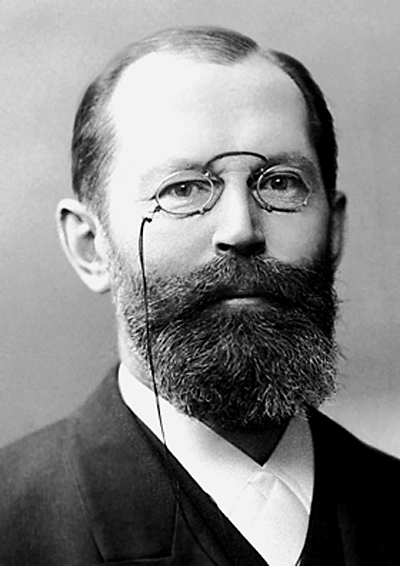
\includegraphics[width=\linewidth]{images/book3/fischer.jpg}
\end{minipage}\hfill
\begin{minipage}[t]{0.78\linewidth}
\vspace{0pt}
حدد إميل فيشر، حتى سنة 1891، الترتيبات الفراغية للغلوكوز ومتماكباته، قبل أن يستطيع أي
منهج فيزيائي رؤية جزيء: بتحويل السكريات بعضها إلى بعض وعدّ
المتماكبات الفراغية الناتجة. والإسقاط الذي ابتكره لكتابتها ما زال يحمل اسمه. وصنع أيضًا
أول ببتيدات صنعية، ونال جائزة نوبل في الكيمياء سنة 1902. (صورة شخصية: أتيلييه
فيكتوريا، برلين، نحو 1895، ملكية عامة؛ ويكيميديا كومنز.)
\end{minipage}
\end{history}

\section{تمارين}

\begin{exercise}[$\star$]\label{exo:b2:biomolecules:1}
ارسم الألانين على هيئة \omterm{def:b2:biomolecules:amino-acid}{أيون مزدوج الشحنة}، ثم الصورتين السائدتين عند pH 1 وعند pH 12.
\end{exercise}

\begin{exercise}[$\star$]\label{exo:b2:biomolecules:2}
احسب \omterm{def:b2:biomolecules:amino-acid}{نقطة التعادل الكهربائي} للغليسين، ونقطة الألانين ($\mathrm pK_a$ 2.35 و9.87).
\end{exercise}

\begin{exercise}[$\star$]\label{exo:b2:biomolecules:3}
ارسم ثنائي \omterm{def:b2:biomolecules:peptide}{الببتيد} Ala--Gly وأحط رابطته الببتيدية بدائرة. بمَ يختلف عن Gly--Ala؟
\end{exercise}

\begin{exercise}[$\star$]\label{exo:b2:biomolecules:4}
في إسقاط فيشر وفيه \ce{COOH} في الأعلى \omterm{def:b2:biomolecules:amino-acid}{والسلسلة الجانبية} \ce{CH2OH} في الأسفل، تتجه
\ce{NH2} في السيرين إلى اليسار. أهو D أم L؟ أعطِ واصف CIP له.
\end{exercise}

\begin{exercise}[$\star\star$]\label{exo:b2:biomolecules:5}
أعطِ الشحنة الصافية \omterm{def:b2:biomolecules:peptide}{للببتيد} الثلاثي Lys--Gly--Asp عند pH 1 و7 و12.
\end{exercise}

\begin{exercise}[$\star\star$]\label{exo:b2:biomolecules:6}
لماذا يُستعمل \omterm{def:b2:biomolecules:peptide}{عامل اقتران} لتكوين \omterm{def:b2:biomolecules:peptide}{رابطة ببتيدية}، بدلًا من \omterm{def:b2:acyl-substitution:derivative}{كلوريد أسيل} الحمض الأميني
المحمي المحضَّر بكلوريد الثيونيل والمسخَّن؟
\end{exercise}

\begin{exercise}[$\star\star$]\label{exo:b2:biomolecules:7}
يتحلق الفركتوز D عبر \ce{OH} على C5 على كيتون C2. أعطِ حجم الحلقة وارسم
$\beta$-D-فركتوفورانوز \omterm{def:b2:biomolecules:anomer}{بإسقاط هاورث}.
\end{exercise}

\begin{exercise}[$\star\star$]\label{exo:b2:biomolecules:8}
\omterm{def:b2:biomolecules:anomer}{للأنوميرين} النقيين للغالاكتوز D دورانان نوعيان $+150.7$ ($\alpha$) و$+52.8$ ($\beta$) 
ولخليط التوازن $+80.2$ (معطيات تمرين). احسب تركيب التوازن.
\end{exercise}

\begin{exercise}[$\star\star$]\label{exo:b2:biomolecules:9}
فسّر لماذا يختزل المالتوز محلول فهلنغ ولا يختزله السكروز، ولماذا يختزله السكروز بعد
التسخين مع حمض مخفف.
\end{exercise}

\begin{exercise}[$\star\star\star$]\label{exo:b2:biomolecules:10}
قرينة \omterm{def:b2:acyl-substitution:saponification}{التصبّن} لدهن هي كتلة هيدروكسيد البوتاسيوم، بوحدة mg، التي \omterm{def:b2:acyl-substitution:saponification}{تصبّن} 1~g منه.
احسبها للتريولين، \ce{C57H104O6}، وفسّر لماذا تكون قيمتها أعلى للدهن ذي السلاسل الأقصر.
\end{exercise}

\begin{exercise}[$\star\star\star$]\label{exo:b2:biomolecules:11}
خطط لتخليق Gly--Ala من الغليسين والألانين: المجموعات الحامية، والتنشيط، والاقتران،
ونزع الحماية، مع زوج متعامد.
\end{exercise}

\begin{exercise}[$\star\star\star$]\label{exo:b2:biomolecules:12}
اكتب الشريط المتمم للشريط \babelsublr{5$'$-ATGCGT-3$'$}، ابتداءً من طرفه \babelsublr{5$'$}، وعُدّ الروابط الهيدروجينية
التي تمسك الشريط المزدوج.
\end{exercise}

\section{مسألة: الأسبارتام}

\begin{problem}[{مسألة نهاية الأسبوع --- الحمضان الأمينيان وترتيباتهما الفراغية، وشحنة
ثنائي الببتيد بدلالة pH، وتخليقه ومشكلة $\alpha$/$\beta$، وحلمهته في مشروب
غازي}]
\label{pb:b2:biomolecules:1}
الأسبارتام هو الإستر الميثيلي لثنائي \omterm{def:b2:biomolecules:peptide}{الببتيد} المتكوّن من المجموعة الكربوكسيلية $\alpha$ لحمض الأسبارتيك L
مع المجموعة الأمينية للفينيل ألانين L. المعطيات: قيم $\mathrm pK_a$ لحمض الأسبارتيك 2.0 و3.9 و9.9 (قيم
نموذجية لمجموعات ثنائي \omterm{def:b2:biomolecules:peptide}{الببتيد}). والكتل المولية (\unit{g/mol}): C 12.011، H 1.008، N 14.007،
O 15.999.
% ledger: use:aspartame, pka:asp1, pka:asp2, pka:asp3, aw:C, aw:H, aw:N, aw:O

\medskip
\noindent\textbf{الجزء الأول --- الحمضان الأمينيان.}
\begin{enumerate}
  \item سمِّ المركبات الثلاثة التي تحررها الحلمهة التامة للأسبارتام.
  \item ارسم حمض الأسبارتيك L والفينيل ألانين L بإسقاط فيشر.
  \item أعطِ واصف CIP لكل مركز فراغي.
  \item كم متماكبًا فراغيًا للأسبارتام؟
  \item ارسم الأسبارتام وعلّم \omterm{def:b2:biomolecules:peptide}{الرابطة الببتيدية} والإستر.
  \item لماذا يكون الترتيب الفراغي لكل حمض أميني مهمًا للطعم الحلو؟
\end{enumerate}

\medskip
\noindent\textbf{الجزء الثاني --- الشحنة بدلالة pH.}
\begin{enumerate}[resume]
  \item عدّد المجموعات القابلة للتأين في الأسبارتام. لماذا لا يكون الطرف C إحداها؟
  \item بالقيم النموذجية، أعطِ الشحنة الصافية عند pH 2.
  \item السؤال نفسه عند pH 7.
  \item السؤال نفسه عند pH 12.
  \item قدّر \omterm{def:b2:biomolecules:amino-acid}{نقطة التعادل الكهربائي} في هذا النموذج.
  \item لماذا تختلف قيم $\mathrm pK_a$ الحقيقية لثنائي \omterm{def:b2:biomolecules:peptide}{الببتيد} عن قيم حمض الأسبارتيك
        الحر؟
\end{enumerate}

\medskip
\noindent\textbf{الجزء الثالث --- التخليق.}
\begin{enumerate}[resume]
  \item لماذا لا يمكن ببساطة تسخين حمض الأسبارتيك مع الإستر الميثيلي للفينيل ألانين معًا؟
  \item أي مجموعات حمض الأسبارتيك يجب حمايتها؟
  \item ماذا يفعل \omterm{def:b2:biomolecules:peptide}{عامل الاقتران} بالمجموعة الكربوكسيلية الحرة؟
  \item لحمض الأسبارتيك مجموعتان كربوكسيليتان. ماذا يتكوّن إذا اقترنت المجموعة الخطأ؟
  \item اقترح حماية متعامدة لا تترك حرة إلا المجموعة الكربوكسيلية $\alpha$، وطريقة
        إزالتها.
  \item لماذا يجب ألا يُترك الحمض الأميني المنشط طويلًا في ظروف قاعدية؟
  \item اكتب تسلسل الخطوات.
\end{enumerate}

\medskip
\noindent\textbf{الجزء الرابع --- الحلمهة في مشروب غازي.}
\begin{enumerate}[resume]
  \item أي روابط الأسبارتام يمكن أن تُحلمه في مشروب حمضي؟ وأيها يتحلمه أولًا؟
  \item أعطِ نواتج حلمهة الإستر وحده.
  \item لماذا يكون مذاق المشروب القديم أقل حلاوة؟
  \item احسب الكتلة المولية للأسبارتام، \ce{C14H18N2O5}.
  \item احسب كمية الأسبارتام في علبة تحوي \qty{180}{mg}.
  \item اذكر كتلة الميثانول المتحرر بالحلمهة التامة لكمية \qty{180}{mg} من
        الأسبارتام.
\end{enumerate}
\end{problem}
